% Où l'on crée les pages à remplir
\documentclass[a4paper,landscape]{article}

% Pour en avoir 4 par page
\paperwidth=0.25\paperwidth
\paperheight=0.25\paperheight
\pdfpagewidth=\paperwidth
\pdfpageheight=\paperheight

\usepackage{tikz}
\usetikzlibrary{quotes,angles}
\usetikzlibrary{positioning}
\usetikzlibrary{calc}%Pour extend line
\usetikzlibrary{math}%Pour définir variables dans Tikz
\usetikzlibrary{arrows.meta} %pour faire des flèches
\usetikzlibrary{babel} % permet d'éviter d'utiliser \shorthandoff{:!}
\usetikzlibrary{decorations.pathmorphing} % Permetr le style fait main sur les figures


\tikzset{ %Pour marquer les perpendiculaires
    right angle quadrant/.code={
        \pgfmathsetmacro\quadranta{{1,1,-1,-1}[#1-1]}     % Arrays for selecting quadrant
        \pgfmathsetmacro\quadrantb{{1,-1,-1,1}[#1-1]}},
    right angle quadrant=1, % Make sure it is set, even if not called explicitly
    right angle length/.code={\def\rightanglelength{#1}},   % Length of symbol
    right angle length=2ex, % Make sure it is set...
    right angle symbol/.style n args={3}{
        insert path={
            let \p0 = ($(#1)!(#3)!(#2)$) in     % Intersection
                let \p1 = ($(\p0)!\quadranta*\rightanglelength!(#3)$), % Point on base line
                \p2 = ($(\p0)!\quadrantb*\rightanglelength!(#2)$) in % Point on perpendicular line
                let \p3 = ($(\p1)+(\p2)-(\p0)$) in  % Corner point of symbol
            (\p1) -- (\p3) -- (\p2)
        }
    }
}

\newcommand{\eq}{Equation}
\newcommand{\mg}{Manga}
\newcommand{\rl}{Relatif}
\newcommand{\pr}{Priorité}
\newcommand{\fr}{Fraction}
\newcommand{\an}{Angles}

\begin{document}
\foreach \mquestion/\mtype in {
    Résoudre \\$3x-7=14$/\eq,
    Résoudre \\$3x+6=2x-1$/\eq,
    Résoudre \\$15x-5+4x=14$/\eq,
    Résoudre \\$3x-7=14$/\eq,
    Résoudre \\$3x-5=x+13$/\eq,
    Résoudre \\$2x+16=4x-8$/\eq,
    Résoudre \\$4(3+x)=40$/\eq,
    Comment s'appelle\\ le bébé du cheval ?/\mg,
    Qu'est-ce que\\ la gogue en\\ équitation ?/\mg,
    Quel est l'oppening\\ de la S4 partie 3\\ de l'Attaque\\ des Titans ?/\mg,
    Quelle est la \\ première chanson \\ de Blackpink ?/\mg,
    Qui a navigué \\ avec Luffy mais \\ n'a pas rejoint\\ l'équipage ? /\mg,
    Quelles sont \\ les évolutions \\ d'Evoli ? /\mg,
    Mao Mao \\ possède-t-elle \\des taches de \\rousseurs ?/\mg,
    Quel est\\ l'opposé\\ de 127 ?/\rl,
    Quel nombre sépare\\ les négatifs\\ des positifs ? /\rl,
    Quel est le symbole\\ des nombres\\ positifs ?/\rl,
    Qui est\\ prioritaire entre \\multiplications\\ et additions ?/\rl,
    Qui est\\ prioritaire entre \\multiplications\\ et divisions ?/\rl,
    Quel est le\\ plus petit entre\\ -12 et -14 ?/\rl,
    Quel est le\\ plus petit entre\\ {-12,4 et -12,32 ?}/\rl,
    Calculer \\ \tiny$5\times(6((2-2)+10)\times27-11)\div3$\normalsize/\pr,
    Calculer \\ \tiny $((6\times9-10)\times10-28)\div3$/\pr,
    Calculer \\ \tiny $(70\div10\times6-10)-29+(-5)$/\pr,
    Calculer \\ \tiny $1+28-4\times 6\div5$/\pr,
    Calculer \\ \tiny $(2+2-2+6-28+29)\times4$/\pr,
    Calculer \\ \tiny $(((3-3)\times7+9)\div3-2)\times7-2$/\pr,
    Calculer \\ \tiny $((28-19)\times11-28+29)\div7\times8$/\pr,
    Calculer \\ \tiny $(243-2)\div1\times2-7$/\pr,
    Calculer \\ $\frac{3}{9}-\frac{14}{45}+\frac{12}{45}$/\fr,
    Calculer \\ $\frac{1}{2}+\frac{1}{3}+\frac{1}{4}+\frac{1}{5}+\frac{1}{6}$/\fr,
    Calculer \\ $\frac{5}{3}-\frac{12}{15}+\frac{18}{30}$/\fr,
    Calculer \\ $\frac{2}{8}+\frac{18}{32}+\frac{15}{64}$/\fr,
    Est-ce que \\ $\frac{8}{0}$ \\ existe ?/\fr,
    Simplifier \\ $\frac{24}{108}$/\fr,
    Simplifier \\ $\frac{60}{100}$/\fr,
    Calculer \\ $\frac{27}{27}+\frac{33}{3}-\frac{18}{6}$/\fr,
    Calculer \\ $\frac{8}{4}+\frac{4}{8}$/\fr,
    Calculer \\ $\frac{17}{4}-\frac{16}{14}$/\fr,
    Calculer \\ $\frac{9}{14}-\frac{9}{126}$/\fr,
    Calculer \\ $\frac{17}{4}-\frac{16}{14}$/\fr,
    Calculer \\ $\frac{20}{8}+\frac{11}{14}$/\fr,
    Combien \\mesure un \\angle plat ?/\an,
    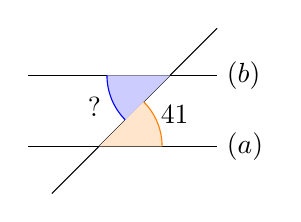
\begin{tikzpicture}[scale=0.6]
            \draw (0,0) coordinate (A1) -- (4,0) coordinate (A2) node[right] {$(a)$};
            \draw (0,1.5) coordinate (B1) -- (4,1.5) coordinate (B2) node[right] {$(b)$};
            \draw (0.5,-1) coordinate (C1) -- (4,2.5) coordinate (C2);
            \node (I1) at (1.5,0) {};
            \node (I2) at (3,1.5) {};
            \draw pic["?",draw=blue,fill=blue!20,angle eccentricity=1.3, angle radius=0.8cm]{angle=B1--I2--I1};
            \draw pic["41",draw=orange,fill=orange!20,angle eccentricity=1.3, angle radius=0.8cm]{angle=A2--I1--I2};
        \end{tikzpicture}
/\an,
    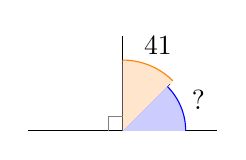
\begin{tikzpicture}[scale=0.6]
            \draw (-2,0) coordinate (A1) -- (0,0) coordinate (I) --(2,0) coordinate (A2) ;
            \draw (I) -- (0,2) coordinate (B);
            \draw (I) -- (1,1) coordinate (C);
            \draw pic["?",draw=blue,fill=blue!20,angle eccentricity=1.3, angle radius=0.8cm]{angle=A2--I--C};
            \draw pic["41",draw=orange,fill=orange!20,angle eccentricity=1.3, angle radius=0.9cm]{angle=C--I--B};
            \draw [gray,right angle quadrant=2,right angle symbol={A1}{A2}{B}];
        \end{tikzpicture}
/\an,
    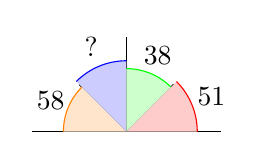
\begin{tikzpicture}[scale=0.6]
            \draw (-2,0) coordinate (A1) -- (0,0) coordinate (I) --(2,0) coordinate (A2) ;
            \draw (I) -- (0,2) coordinate (C);
            \draw (I) -- (1,1) coordinate (D);
            \draw (I) -- (-1,1) coordinate (B);
            \draw pic["58",draw=orange,fill=orange!20,angle eccentricity=1.3, angle radius=0.8cm]{angle=B--I--A1};
            \draw pic["?",draw=blue,fill=blue!20,angle eccentricity=1.3, angle radius=0.9cm]{angle=C--I--B};
            \draw pic["38",draw=green,fill=green!20,angle eccentricity=1.3, angle radius=0.8cm]{angle=D--I--C};
            \draw pic["51",draw=red,fill=red!20,angle eccentricity=1.3, angle radius=0.9cm]{angle=A2--I--D};
        \end{tikzpicture}/\an,
    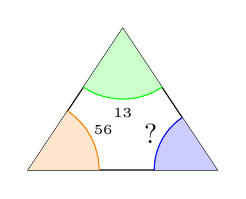
\begin{tikzpicture}[scale=0.6]
            \draw (-2,0) coordinate (A) -- (2,0) coordinate (B)--(0,3) coordinate (C)--cycle;
            \draw pic["?",draw=blue,fill=blue!20,angle eccentricity=1.2, angle radius=0.8cm]{angle=C--B--A};
            \draw pic["\tiny{56}",draw=orange,fill=orange!20,angle eccentricity=1.2, angle radius=0.9cm]{angle=B--A--C};
            \draw pic["\tiny{13}",draw=green,fill=green!20,angle eccentricity=1.2, angle radius=0.9cm]{angle=A--C--B};
        \end{tikzpicture}/\an,
    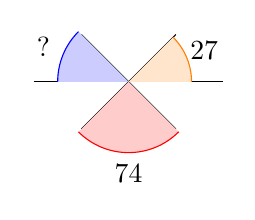
\begin{tikzpicture}[scale=0.6]
            \draw (-2,0) coordinate (A1) -- (0,0) coordinate (I) --(2,0) coordinate (A2) ;
            \draw (I) -- (1,-1) coordinate (D);
            \draw (I) -- (1,1) coordinate (C);
            \draw (I) -- (-1,1) coordinate (B);
            \draw (I) -- (-1,-1) coordinate (E);
            \draw pic["27",draw=orange,fill=orange!20,angle eccentricity=1.3, angle radius=0.8cm]{angle=A2--I--C};
            \draw pic["?",draw=blue,fill=blue!20,angle eccentricity=1.3, angle radius=0.9cm]{angle=B--I--A1};
            \draw pic["74",draw=red,fill=red!20,angle eccentricity=1.3, angle radius=0.9cm]{angle=E--I--D};
        \end{tikzpicture}/\an
}
{
    \newpage %Front side
    \pagecolor{white}%
    \begin{tikzpicture}[remember picture,overlay] % Pour un positionnement précis sur la page
        \node[font=\bfseries,scale=1.9,yshift=0.8mm,align=center] at (current page) {\mquestion} ;
        %\node[anchor=north east] at (current page.north east) % Si on veut rajouter une déco dans un coin
    \end{tikzpicture}
    \newpage %Back side
    \begin{tikzpicture}[remember picture,overlay]
        \node[font=\bfseries,scale=4.5,yshift=0.8mm] at (current page) {\mtype} ;% front side
        \node[font=\bfseries,scale=2,yshift=-4mm] at (current page) {Classe de 5H}; % back side
        \node[font=\bfseries,scale=1,yshift=-2cm] at (current page) {2024-2025}; % back side
    \end{tikzpicture}
    \renewcommand{\eq}{green!60} % Pour avoir les couleurs associées aux types de question
    \renewcommand{\mg}{yellow}
    \renewcommand{\rl}{cyan!50}
    \renewcommand{\pr}{orange}
    \renewcommand{\an}{violet!80}
    \renewcommand{\fr}{magenta!80}
    \pagecolor{\mtype}%
}
%%%%%%%% Le code initial piqué sur StackExchange
% \newcount\malc 
% \malc=0
% \loop
% \advance\malc by 1
% \foreach \mcolor/\mside in {white/front,pink/Classe de 5H 2025}
% {
%     \newpage
%     \pagecolor{\mcolor}%
%     \begin{tikzpicture}[remember picture,overlay]
%         \node[font=\bfseries,scale=10,yshift=0.8mm] at (current page) {\the\malc} ;% front side
%         \node[font=\bfseries,scale=2,yshift=-4mm] at (current page) {\mside{} }; % back side
%     \end{tikzpicture}
% }
% \ifnum\malc<32\repeat % Pour répéter la boucle loop
\end{document}